\documentclass[a5paper,14pt,titlepage,extrafontsizes]{memoir}
\usepackage[a5paper,margin=1cm,showframe]{geometry}
\usepackage{color}
\usepackage{background}
\usepackage{helvet}
\usepackage[utf8]{inputenc}
\usepackage{outline}
\renewcommand*{\familydefault}{\sfdefault}
\usepackage[outline]{contour}
\contourlength{.3pt}

\backgroundsetup{
scale=1,
angle=0,
opacity=1.0,  %% adjust
contents={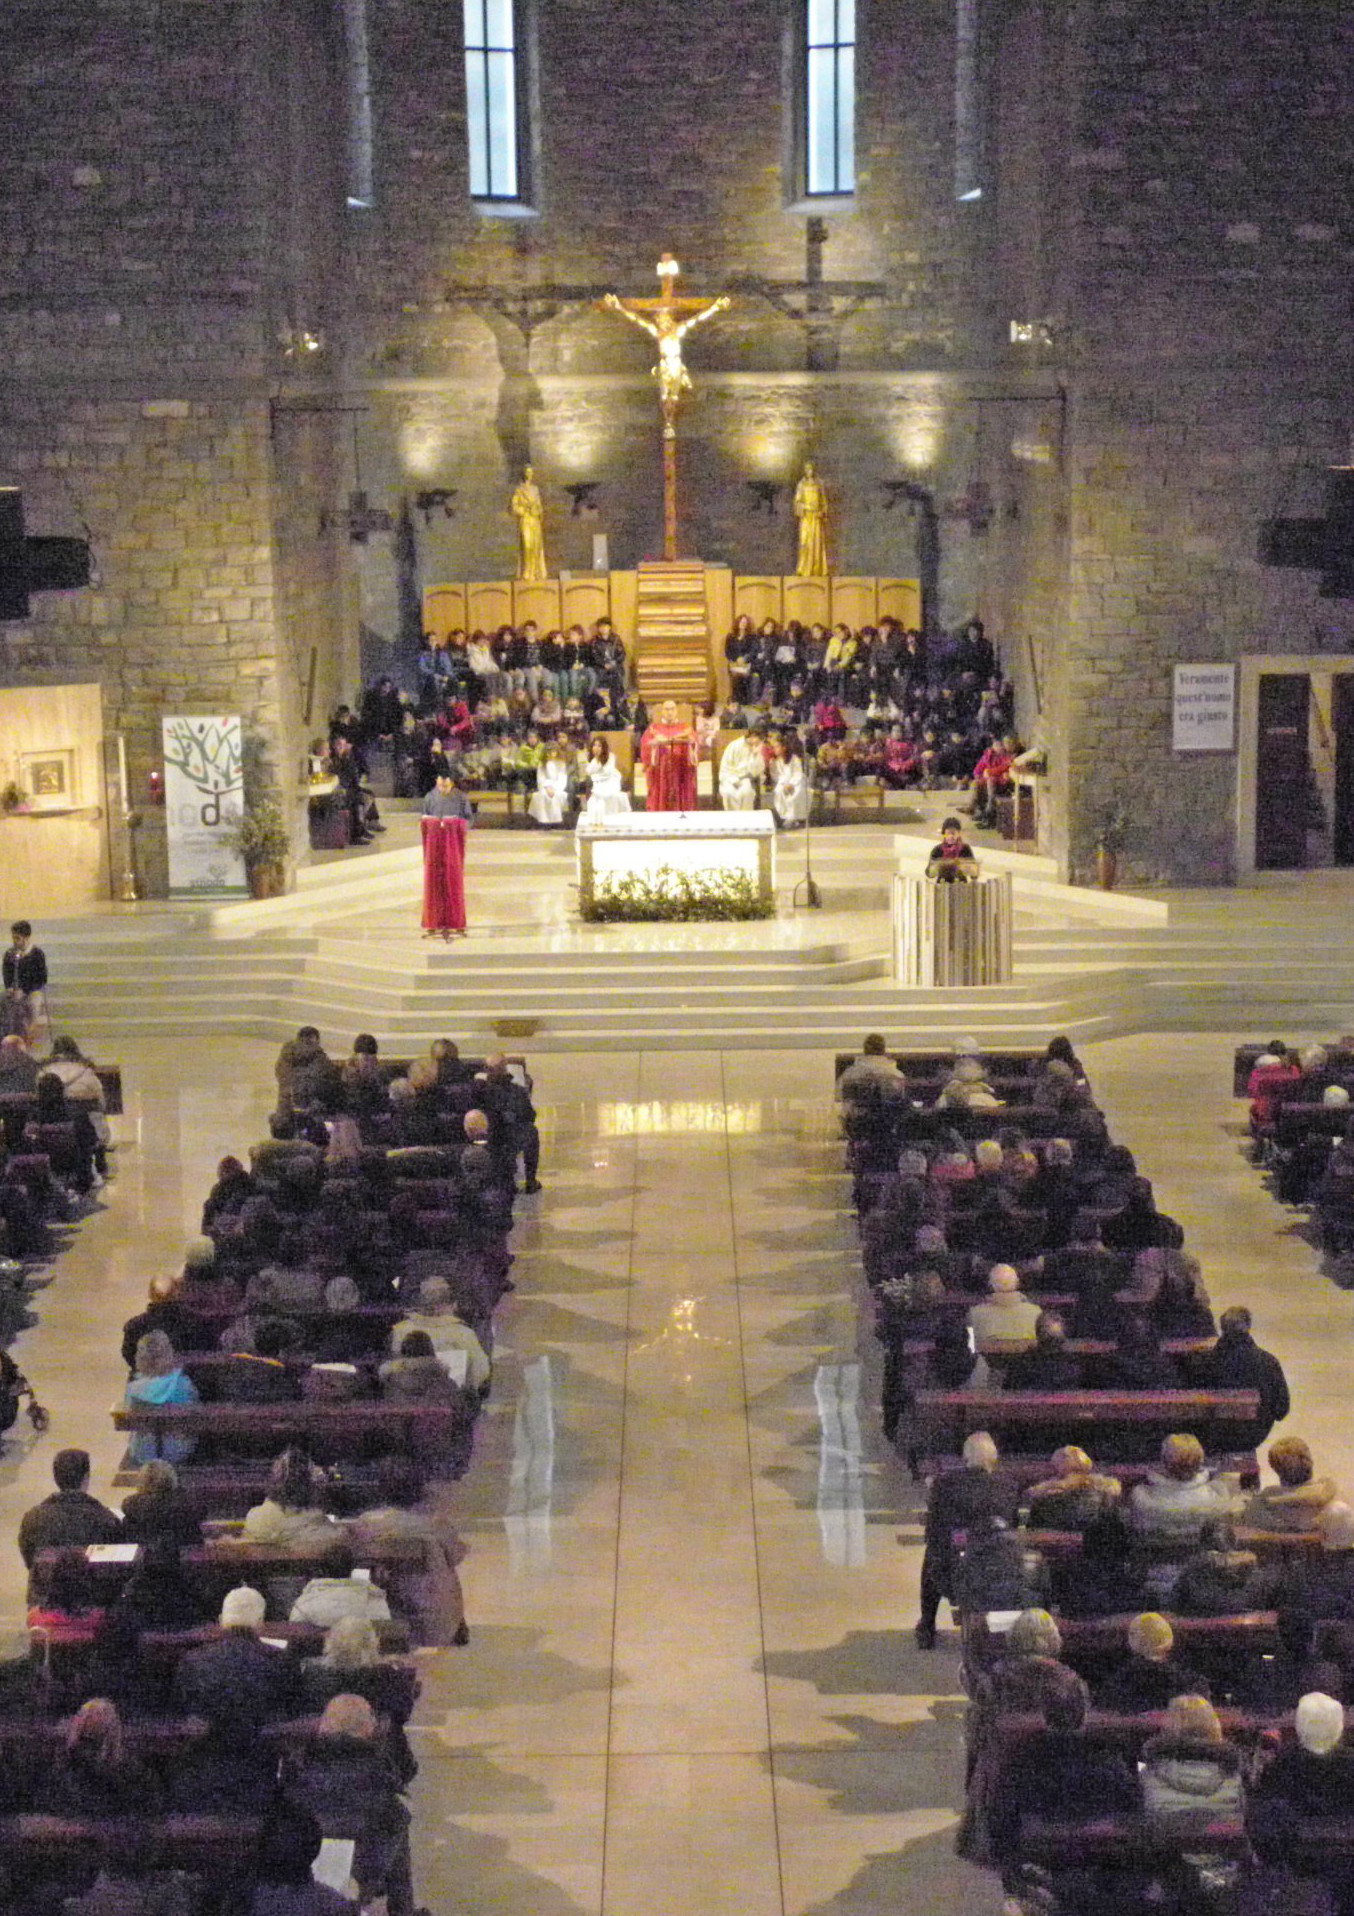
\includegraphics[width=\paperwidth,height=\paperheight ]{chiesa}}
}
\begin{document}
\pagestyle{empty}
\begin{center}
 \vspace*{\fill}
 {\Huge\color{white}\contour{black}{PARROCCHIA di}\\\contour{black}{SAN FRANCESCO}\\[20pt] \contour{black}{in TRIESTE}}\\[25pt]
 {\Large\color{white}\bfseries \contour{black}{2015: 50 ANNI di VITA}}\\[10pt]
 {\Large\color{white}\itshape  \contour{black}{la comunità racconta}}
 \vspace{0pt}
\end{center}
\newpage
\end{document}